\printconcepts

\exercise{Why is sketching curves by hand beneficial even though technology is readily available?}{Answers will vary.}

\exercise{T/F: When sketching graphs of functions, it is useful to find the critical points.}{T}

\exercise{T/F: When sketching graphs of functions, it is useful to find the possible points of inflection.}{T}

\exercise{T/F: When sketching graphs of functions, it is useful to find the horizontal and vertical asymptotes.}{T}

\printproblems

\exercise{Given the graph of $f$, identify the concavity of $f$, its inflection points, its regions of increasing and decreasing, and its relative extrema.\\
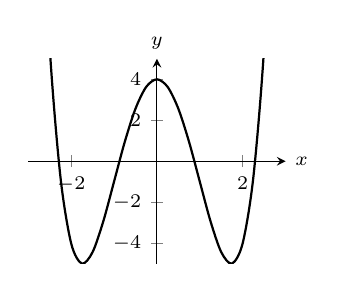
\begin{tikzpicture}
\begin{axis}[width=.4\textwidth,tick label style={font=\scriptsize },
	axis y line=middle,axis x line=middle,
    ymin=-5,ymax=5,
	xmin=-3,xmax=3,name=myplot]
\addplot [{\colorone},smooth,thick,domain=-3:3] {x^2*(x^2-6)+4};
\end{axis}
\node [right] at (myplot.right of origin) {\scriptsize $x$};
\node [above] at (myplot.above origin) {\scriptsize $y$};
\end{tikzpicture}}{concave up on $(-\infty,-1)$; $(1,\infty)$\\
concave down on $(-1,1)$\\
inflection points when $x=\pm1$\\
increasing on $(-2,0)$; $(2,\infty)$\\
decreasing on $(-\infty,-2)$; $(0,2)$\\
relative maximum when $x=0$\\
relative minima when $x=\pm2$}

\exercise{Given the graph of $\fp$, identify the concavity of $f$, its inflection points, its regions of increasing and decreasing, and its relative extrema.\\
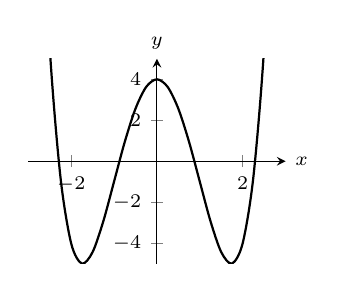
\begin{tikzpicture}
\begin{axis}[width=.4\textwidth,tick label style={font=\scriptsize },
	axis y line=middle,axis x line=middle,
    ymin=-5,ymax=5,
	xmin=-3,xmax=3,name=myplot]
\addplot [{\colorone},smooth,thick,domain=-3:3] {x^2*(x^2-6)+4};
\end{axis}
\node [right] at (myplot.right of origin) {\scriptsize $x$};
\node [above] at (myplot.above origin) {\scriptsize $y$};
\end{tikzpicture}}{concave up on $(-2,0)$; $(2,\infty)$\\
concave down on $(-\infty,-2)$; $(0,2)$\\
inflection points when $x=0,\pm2$\\
increasing on $(-\infty,-2.3)$; $(-1,1)$; $(2.3,\infty)$\\
decreasing on $(-2.3,-1)$; $(1,2.3)$\\
relative maximum when $x=-2.3,1$\\
relative minima when $x=-1,2.3$}

\exercise{Sketch the graph of a function that is\\
concave up on $(-\infty,-1)$; $(1,\infty)$;\\
concave down on $(-1,1)$;\\
increasing on $(-\infty,0)$; and\\
decreasing on $(0,\infty)$.}{various possibilities}

\input{exercises/03_05_exset_01}

{\noindent In Exercises}
{, sketch a graph of the given function using Key Idea \ref{idea:sketch}. Show all work; check your answer with technology.
}
\exinput{exercises/03_05_ex_12}
\exinput{exercises/03_05_ex_13}
\exinput{exercises/03_05_ex_14}
\exinput{exercises/03_05_ex_15}
\exinput{exercises/03_05_ex_16}
\exinput{exercises/03_05_ex_17}
\exinput{exercises/03_05_ex_18}
\exinput{exercises/03_05_ex_19}
\exinput{exercises/03_05_ex_34}
\exinput{exercises/03_05_ex_20}
\exinput{exercises/03_05_ex_21}
\exinput{exercises/03_05_ex_22}
\exinput{exercises/03_05_ex_23}
\exinput{exercises/03_05_ex_24}
\exinput{exercises/03_05_ex_25}
\exinput{exercises/03_05_ex_30}
\exinput{exercises/03_05_ex_39}
\exinput{exercises/03_05_ex_31}
\exinput{exercises/03_05_ex_32}
\exinput{exercises/03_05_ex_33}
\exinput{exercises/03_05_ex_38}


\begin{exerciseset}{In Exercises}{, a function with the parameters $a$ and $b$ are given. Describe the critical points and possible points of inflection of $f$ in terms of $a$ and $b$.}

\exercise{$\ds f(x) = \frac{a}{x^2+b^2}$}{Critical point: $x=0$; Points of inflection: $\pm b/\sqrt{3}$}

\exercise{$f(x)=ax^2+bx+1$}{Critical point: $x=-b/2a$; Points of inflection: none}

\exercise{$\ds f(x) = \sin (ax+b)$}{Critical points: $x=\frac{n\pi/2-b}{a}$, where $n$ is an odd integer; Points of inflection: $(n\pi-b)/a$, where $n$ is an integer.}

\exercise{$\ds f(x) = (x-a)(x-b)$}{Critical point: $x=(a+b)/2$; Points of inflection: none}

\end{exerciseset}


\exercise{Given $x^2+y^2=1$, use implicit differentiation to find $\dfrac{dy}{dx}$ and $\dfrac{d^2y}{dx^2}$. Use this information to justify the sketch of the unit circle.
}{$\dfrac{dy}{dx} = -x/y$, so the function is increasing in second and fourth quadrants, decreasing in the first and third quadrants.

$\dfrac{d^2y}{dx^2} = -1/y^3$, which is positive when $y<0$ and is negative when $y>0$. Hence the function is concave down in the first and second quadrants and concave up in the third and fourth quadrants.}
